% Generated by thesis/ch7/exp2/exp2_figures.py -- do not edit by hand.
\begin{figure}[tbp]
  \centering
  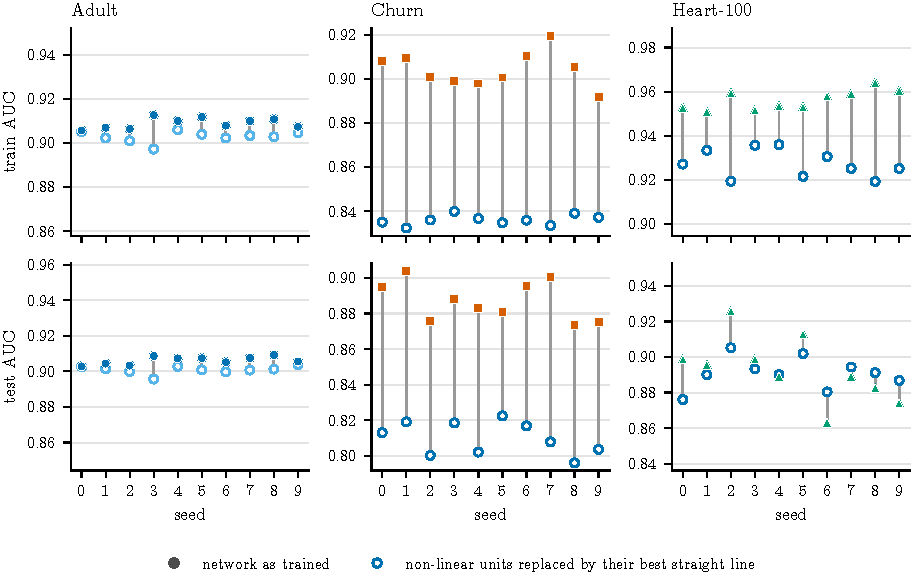
\includegraphics[width=\textwidth,height=0.8\textheight,keepaspectratio]{figures/ch7/options/linearised-auc}
  \caption{AUC of each network as trained and with its non-linear units linearised. Filled: the network as trained; open: every non-linear unit replaced by its best straight line; grey: joins a seed's two values. The panels of a row span the same AUC range.}
  \label{fig:ch7-linearised-auc}
\end{figure}
